\section{Performance Evaluation}\label{sec:perf}

The PBBS benchmark consists of three data sets. Each of these consists of
$10^8$ points drawn from different distributions. Even though all data sets
are $1.6$ GB in size, the algorithm behaves very differently on them.

\tkcomment{Move to related work?}
As a baseline we have considered Qhull \cite{}, the algorithms of CGAL \cite{},
and the implementation of PBBS. Some preliminary testing shows that the
implementation of PBBS is the fastest by a large margin. In
Table~\ref{table:reference} are the runtimes for a disk of $10^7$ points.

\begin{table}[ht]
    \caption{Runtime in seconds for a disk of $10^7$ points}
    \label{table:reference}
    \begin{tabular}{c | c }
     Implementation & Runtime \\ 
     \hline \\
     PBBS & 0.31 \\  
     CGAL Quickhull & 0.61 \\
     CGAL Akl-Toussaint & 0.60 \\
     CGAL Bykat & 0.73 \\
     CGAL Eddy & 0.98 \\
     CGAL Graham & 1.3 \\
     CGAL Jarvis & 208 \\
     Qhull & 1.1 \\
    \end{tabular}
\end{table}

We use GCC 14.1.1. All experiments are run 20 times. The standard deviation is 
less than $2.5\%$ in all cases, so we only report the means.

\subsection{Evaluation Platforms}

We evaluate our implementation on two machines. The first, \textit{cn125}
has powerful vector instructions, a modest amount of cores and memory, and a 
simple memory architecture. 

The second, \textit{cn132}, has less powerful vector instructions and needs
to implement the compression instruction in software. It has two CPUs which
gives it more cores and memory bandwidth. Memory is local to one of the two
CPUs, so we need to make sure allocations are equally distributed between the
two. We have done this by running the programs under
\texttt{numactl --interleaved all}.

We summarize the systems in Table~\ref{tab:system}. There can be a significant
gap between the bandwidth the RAM is capable off, and what is achievable in
practice. The STREAM benchmark \cite{McCalpin95} is a collection of simple
functions that can be used to measure what bandwidths can be attained 
practically. We obtained the best results by pinning threads to cores and 
disabling hyperthreading.

\begin{table}[ht]
    \caption{Theoretical and practical capabilities of test systems. All four
             STREAM benchmarks obtained the same bandwidth.}
    \label{tab:system}
    \begin{tabular}{c|c|c}
                                   & cn132 & cn125          \\
        \hline                                              
        CPU                        & Epyc 7313 $(\times 2)$ 
                                           & Xeon E-2378    \\
        Vector extension           & AVX2  & AVX-512        \\
        Frequency (GHz)            & 3.7   & 2.6            \\
        Peak compute rate (Gflops) & 1894  & 346            \\
        Theoretic bandwidth (GB/s) & 204.8 & 51.2           \\ 
        STREAM (GB/s)              & 140   & 41             \\ 
    \end{tabular}
\end{table}

\subsection{The Data Sets}\label{subsec:datasets}

There is a large difference between runtime of Quickhull on the different 
datasets.

\subsubsection{Kuzmin}

Whereas Circle and Disk are symmetric, Kuzmin is very much the opposite
as illustrated in Figure~\ref{fig:kuzmin}.
The first two partitions end up with almost all points either in $S_1$ or
in $S_2$, and on the subsequent partition almost all points are discarded.
The convex hull has only $4$ points.

\begin{figure}[ht]
    \centering
    \includegraphics[width=0.5\textwidth]{./figures/rust-kuzmin.png}
    \caption{The Kuzmin dataset of $10^8$ points. The first partition only
             moves $r_1$. The second partition eliminates all remaining points.}
    \label{fig:kuzmin}
\end{figure}

\subsubsection{Circle}

A circle is convex, so all points are on the hull. As a circle is symmetric,
each recursive call of FindHull will identify one element on the hull, and
then recurse on two subsets $S_1$ and $S_2$ differing at most one in size.
That means we have a deep recursion.

\textbf{A note on accuracy: }the actual dataset is only an approximation of
a circle, and we classify roughly one in ten points as lying on the convex
hull. Both implementations find the same points up to $10^7$ points, but on 
$10^8$ they disagree on $20$ points. These are points $u$ for which 
$\text{orient}(p, u, r_1) > 0$ and $\text{orient}(r_2, u, q) > 0$ which
can only happen due to round-off error. We have made the arbitrary decision
to put these in $S_1$.

\subsubsection{Disk}

The first recursion will identify $p$, $r_1$, $q$, $r_2$ as lying on the
convex hull, and partition the points into those above and below $pq$.
Then the second partition will eliminate region V of 
Figure~\ref{fig:disk_level2}. This square has area $2$, so it will eliminate
most points: a fraction $\frac{2}{\pi} \approx 0.637$.

\begin{figure}[ht]
    \begin{subfigure}{0.4\textwidth}
        \resizebox{\columnwidth}{!}{%
        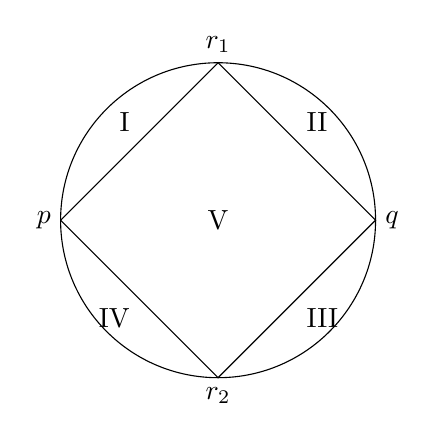
\begin{tikzpicture}
            \draw (0, 0) circle (2);
            \draw (-2, 0) node[left]  {$p$}   -- node[pos=0.5, above left] {I}
                  (0, 2)  node[above] {$r_1$} -- node[pos=0.5, above right] {II}
                  (2, 0)  node[right] {$q$}   -- node[pos=0.5, below right] {III}
                  (0, -2) node[below] {$r_2$} -- node[pos=0.5, below left] {IV}
                  (-2, 0);
              \node at (0, 0) {V};
        \end{tikzpicture}}
        \caption{The Disk data set at recursion level 2. Region V will be 
                 eliminated, and the recursion will continue on regions I 
                 \textemdash IV.}
        \label{fig:disk_level2}
    \end{subfigure}
    \hfill
    \begin{subfigure}{0.4\textwidth}
        \resizebox{\columnwidth}{!}{%
        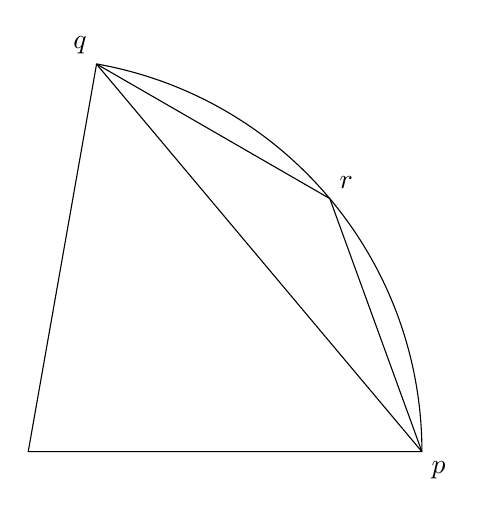
\begin{tikzpicture}
            \foreach \r in {5} {
            \draw (0,0) arc (0:80:\r);
            \draw (0,0)  node[below right] {$p$} -- ++(0+180:\r) -- 
                                +(80:\r) node[above left] {$q$};
            \draw (0.766 * \r - 1 * \r, 0.6428 * \r) node[above right] {$r$};
            \draw (0.173 * \r - 1 * \r, 0.985 * \r) -- (0, 0);
            \draw (0.173 * \r - 1 * \r, 0.985 * \r) -- 
                  (0.766 * \r - 1 * \r, 0.6428 * \r) -- (0, 0);
        }
        \end{tikzpicture}}
        \caption{Subset of Disk we apply a recursive call of the Quickhull 
                 algorithm on. The points are uniformly sampled from the disk
                 segment to the right of the line segment $rs$.}
        \label{fig:disk_level3+}
    \end{subfigure}
    \caption{Quickhull on Disk dataset at different recursion levels.}
\end{figure}

After this, the recursion will continue on pie slices of progressively smaller
angle (Figure~\ref{fig:disk_level3+}. 
The proportion of points eliminated is almost constant in this angle and roughly
equal to $0.74$.
%To see this, we label some points in Figure~\ref{fig:disk_level3+}. 

%The elements not yet eliminated lie to the right of $rs$, and in this step,
%we eliminate the elements in $\Delta rqs$.
%
%The triangle $\Delta prs$ is isosceles, so $\angle par$ and $\angle pas$
%are right angles. That gives us $|pa| = \cos(\theta / 2)$ and 
%$|sa| = |ar| = \sin(\theta / 2)$. So $\Delta psr$ has area 
%$\sin(\theta / 2) \cos(\theta / 2) = \frac{1}{2} \sin(\theta)$. The entire
%pie slice has area $\frac{\theta}{2 \pi} \cdot \pi = \frac{1}{2} \theta$.
%Therefore, the part of the circle above the line $rs$ has area 
%$\frac{1}{2}(\theta - \sin(\theta))$.
%
%Since $|aq| = |pq| - |pa| = 1 - \cos(\theta / 2)$, the area of $\Delta rqs$
%is $\sin(\theta / 2) (1 - \cos(\theta / 2))$. So the fraction of points we
%eliminate is
%
%$$\frac{2\sin(\theta / 2) (1 - \cos(\theta / 2))}{\theta - \sin(\theta)}.$$
%
%We approximate this with a third degree Chebyshev approximation on 
%$[0, \frac{\pi}{2}]$, which is
%
% 1.48202191816423201 * 0.5 - -0.00314946736514754 = 0.744160426447263545
% -0.01207255984434141 - 3 * -0.00007573579005338  = -0.01184535247418127
% 2 * -0.00314946736514754                         = -0.00629893473029508
% 4 * -0.00007573579005338                         = -0.00030294316021352
%$$0.744 - 0.012 \theta - 0.0063 \theta^2 - 0.0003 \theta^3. $$
%
%The smaller $\theta$ gets, the closer this will be to $0.744$. Even for the
%largest $\theta = \frac{\pi}{2}$, this value is reasonably close: $0.708$. 
%So we take $0.74$ as approximation. That means the recursion depth is roughly
%$1 + \log_{\frac{1}{1 - 0.74}}((1 - 0.637) \cdot 10^8) \approx 14$.
%
%The convex hull has $1593$ points.

\subsection{Interpreting the Results}

Evaluating the performance of an algorithm and its implementation is difficult.
The runtime alone tells us little about the quality of the implementation, as
it differs between machines.

For this reason we also compute the bandwidth. Assuming a double is $8$ bytes,
this is $8n$ bytes for finding the left-most and right-most points. At each
recursive call, we have $8(n + |S_1| + |S_2|)$ bytes for the partition,
and $8|CH(S_2)|$ bytes to place $CH(S_1)$ and $CH(S_2)$ next to each other in
memory. This is $5.6$ GB, $73$ GB, $7.2$ GB for Kuzmin, Circle, and Disk.

The data movement of our algorithm is not optimal. Take for example Disk:
The Akl-Toussaint heuristic \cite{akl78} lets us identify $p_1, \cdots, p_8$
of Figure~\ref{fig:akl} in one pass. This octagon has area $2\sqrt{2}$,
which is approximately $90\%$ of the disk, and these points can be eliminated.

Points $u$ satisfy $orient(p_i, u, p_{i + 1 \text{ mod } 8}) > 0$ for precisely 
one $i$ if they are between the circle and line segment 
$\overrightarrow{p_i p_{i + 1 \text{ mod } 8}}$, or none if 
$u$ is inside the octagon.
If we can partition the input into these eight areas
in one pass as well, we need only $1.6 + 1.6 + 0.16 = 3.36$ GB to eliminate
$90\%$ of points. Our algorithm gets to the same points in $3$ levels of
recursion, which takes $6.5$ GB. So a better algorithm can cut the required
bandwidth almost in half. To take this into account we also look at the minimum
amount of data movement any algorithm can obtain: the size of the input plus
the size of the output. Dividing this by the runtime is called the
\textit{effective bandwidth}.

\begin{figure}[ht]
    \resizebox{\columnwidth}{!}{%
    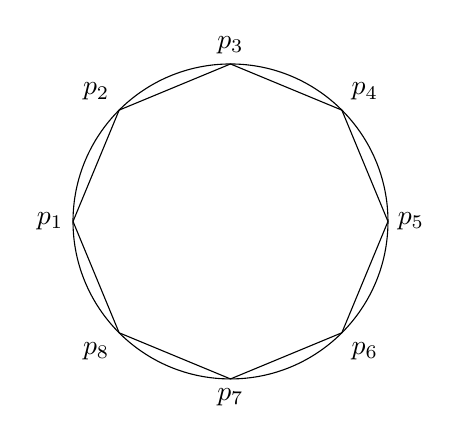
\begin{tikzpicture}
        \draw (0, 0) circle (2);
        \draw (-2, 0) node[left] {$p_1$} --
              (-1.414, 1.414) node[above left] {$p_2$} --
              (0, 2) node[above] {$p_3$} --
              (1.414, 1.414) node[above right] {$p_4$} --
              (2, 0) node[right] {$p_5$} --
              (1.414, -1.414) node[below right] {$p_6$} --
              (0, -2) node[below] {$p_7$} --
              (-1.414, -1.414) node[below left] {$p_8$} --
              (-2, 0);
    \end{tikzpicture}}
    \caption{Points $p_1, \cdots, p_8$ can be found by minimum / maximum
             $x$-coordinates, $y$-coordinates, differences / sums of 
             $x$ and $y$ coordinates. Points within this octagon are not in 
             the convex hull.}
    \label{fig:akl}
\end{figure}

\subsection{Analysis}

In contrast to our approach, PBBS does not permute the points, but instead
an array of indices pointing to the subsets. This can make for poor spatial
locality in the access of $P$, especially in deeper recursion levels.
It also inhibits vectorization.

For the Kuzmin, almost all points belong in either $S_1$ or $S_2$, so
this dataset is the exception. Similarly, the branches are easy to predict,
giving VecQuickhull little advantage over the approach of
PBBS. For this reason, we see in Table~\ref{table:runtime} that the deeper
the recursion, the larger our lead over PBBS becomes. 

Kuzmin has to get its data from RAM in all its passes, so we can expect
at most the bandwidth obtained by the STREAM benchmark. We see in 
Table~\ref{table:bw} that we get closer ($83\%$) to STREAM 
on cn125, than on cn132 ($67\%$). We speculate that the hardware prefetcher
is less effective on our more complicated access pattern.
Circle has a deep recursion, which means it can use the caches effectively. This
leads to high bandwidth, but low effective bandwidth (Table~\ref{table:ef_bw}).

% Generated with scripts

\pgfplotstableread{
Imp,Kuzmin,kuzminstd,Circle,circlestd,Disk,diskstd
PBBS,9.80e-01, 1.38e-03, 6.11e+01, 1.72e-01, 3.86e+00, 1.07e-02
VecQuickhull,2.93e-01, 1.23e-03, 4.73e+00, 1.19e-02, 4.48e-01, 1.96e-03
PBBS par,2.34e-01, 2.74e-03, 8.71e+00, 5.85e-02, 5.29e-01, 9.97e-03
VecQuickhull par,1.60e-01, 3.62e-03, 1.07e+00, 1.17e-02, 2.12e-01, 3.41e-03
}\runtimetable

\pgfplotstableread{
Imp,Kuzmin,kuzminstd,Circle,circlestd,Disk,diskstd
PBBS,6.88e-01, 3.89e-03, 5.43e+01, 1.13e-01, 3.59e+00, 1.75e-02
VecQuickhull,4.39e-01, 3.45e-03, 6.57e+00, 1.54e-02, 6.74e-01, 4.47e-03
PBBS par,7.40e-02, 4.24e-04, 3.24e+00, 1.91e-02, 1.90e-01, 3.41e-03
VecQuickhull par,5.72e-02, 2.56e-03, 3.78e-01, 2.60e-02, 9.02e-02, 1.59e-02
}\runtimetablenuma

\pgfplotstableread{
Imp,Kuzmin,kuzminstd,Circle,circlestd,Disk,diskstd
PBBS,5.71e+00, 4.04e+03, 1.19e+00, 4.23e+02, 1.86e+00, 6.73e+02
VecQuickhull,1.91e+01, 4.54e+03, 1.54e+01, 6.15e+03, 1.61e+01, 3.67e+03
PBBS par,2.39e+01, 2.05e+03, 8.38e+00, 1.25e+03, 1.36e+01, 7.22e+02
VecQuickhull par,3.50e+01, 1.55e+03, 6.81e+01, 6.26e+03, 3.40e+01, 2.11e+03
}\bwtable

\pgfplotstableread{
Imp,Kuzmin,kuzminstd,Circle,circlestd,Disk,diskstd
PBBS,8.13e+00, 1.44e+03, 1.35e+00, 6.46e+02, 2.00e+00, 4.10e+02
VecQuickhull,1.27e+01, 1.62e+03, 1.11e+01, 4.73e+03, 1.07e+01, 1.61e+03
PBBS par,7.57e+01, 1.32e+04, 2.26e+01, 3.82e+03, 3.79e+01, 2.11e+03
VecQuickhull par,9.79e+01, 2.19e+03, 1.93e+02, 2.81e+03, 7.98e+01, 4.53e+02
}\bwtablenuma

\pgfplotstableread{
Imp,Kuzmin,kuzminstd,Circle,circlestd,Disk,diskstd
PBBS,1.63e+00, 1.16e+03, 2.64e-02, 9.35e+00, 4.14e-01, 1.50e+02
VecQuickhull,5.46e+00, 1.30e+03, 3.41e-01, 1.36e+02, 3.58e+00, 8.16e+02
PBBS par,6.84e+00, 5.85e+02, 1.85e-01, 2.75e+01, 3.02e+00, 1.60e+02
VecQuickhull par,9.99e+00, 4.42e+02, 1.50e+00, 1.38e+02, 7.55e+00, 4.70e+02
}\efbwtable

\pgfplotstableread{
Imp,Kuzmin,kuzminstd,Circle,circlestd,Disk,diskstd
PBBS,2.32e+00, 4.12e+02, 2.97e-02, 1.43e+01, 4.45e-01, 9.12e+01
VecQuickhull,3.64e+00, 4.64e+02, 2.45e-01, 1.04e+02, 2.38e+00, 3.58e+02
PBBS par,2.16e+01, 3.77e+03, 4.98e-01, 8.43e+01, 8.41e+00, 4.70e+02
VecQuickhull par,2.80e+01, 6.25e+02, 4.26e+00, 6.19e+01, 1.77e+01, 1.01e+02
}\efbwtablenuma

\tkcomment{For some reason it is really hard to get significant figures
in Latex. Maybe write a C program that generates Latex code.}

\begin{table}[ht]
    \caption{VecQuickhull and PBBS Quickhull runtime in seconds on cn125.}
    \label{table:runtime}
    \pgfplotstabletypeset[
        columns={Imp,Kuzmin,Circle,Disk},
        column type/.add={|}{},
        every last column/.style={column type/.add={}{|}},
        every head row/.style={before row=\hline, after row=\hline},
        every last row/.style={after row=\hline},
        columns/Imp/.style={string type, column name={}},
    ]\runtimetable
\end{table}

\begin{table}[ht]
    \caption{VecQuickhull and PBBS Quickhull runtime in seconds on cn132.}
    \label{table:runtimenuma}
    \pgfplotstabletypeset[
        columns={Imp,Kuzmin,Circle,Disk},
        column type/.add={|}{},
        every last column/.style={column type/.add={}{|}},
        every head row/.style={before row=\hline, after row=\hline},
        every last row/.style={after row=\hline},
        columns/Imp/.style={string type, column name={}},
    ]\runtimetablenuma
\end{table}

\begin{table}[ht]
    \caption{VecQuickhull and PBBS Quickhull bandwidth in GB/s on cn125.}
    \label{table:bw}
    \pgfplotstabletypeset[
        columns={Imp,Kuzmin,Circle,Disk},
        column type/.add={|}{},
        every last column/.style={column type/.add={}{|}},
        every head row/.style={before row=\hline, after row=\hline},
        every last row/.style={after row=\hline},
        columns/Imp/.style={string type, column name={}},
    ]\bwtable
\end{table}

\begin{table}[ht]
    \caption{VecQuickhull and PBBS Quickhull bandwidth in GB/s on cn132.}
    \label{table:bwnuma}
    \pgfplotstabletypeset[
        columns={Imp,Kuzmin,Circle,Disk},
        column type/.add={|}{},
        every last column/.style={column type/.add={}{|}},
        every head row/.style={before row=\hline, after row=\hline},
        every last row/.style={after row=\hline},
        columns/Imp/.style={string type, column name={}},
    ]\bwtablenuma
\end{table}


\begin{table}[ht]
    \caption{VecQuickhull and PBBS Quickhull effective bandwidth in GB/s
             on cn125.}
    \label{table:ef_bw}
    \pgfplotstabletypeset[
        columns={Imp,Kuzmin,Circle,Disk},
        column type/.add={|}{},
        every last column/.style={column type/.add={}{|}},
        every head row/.style={before row=\hline, after row=\hline},
        every last row/.style={after row=\hline},
        columns/Imp/.style={string type, column name={}},
        columns/Kuzmin/.style={fixed},
        columns/Circle/.style={fixed},
        columns/Disk/.style={fixed},
    ]\efbwtable
\end{table}

\begin{table}[ht]
    \caption{VecQuickhull and PBBS Quickhull effective bandwidth in GB/s
             on cn132.}
    \label{table:ef_bwnuma}
    \pgfplotstabletypeset[
        columns={Imp,Kuzmin,Circle,Disk},
        column type/.add={|}{},
        every last column/.style={column type/.add={}{|}},
        every head row/.style={before row=\hline, after row=\hline},
        every last row/.style={after row=\hline},
        columns/Imp/.style={string type, column name={}},
        columns/Kuzmin/.style={fixed},
        columns/Circle/.style={fixed},
        columns/Disk/.style={fixed},
    ]\efbwtablenuma
\end{table}
